\documentclass{article}

\usepackage[utf8]{inputenc}
\usepackage[brazilian]{babel}
\usepackage{graphicx}
\usepackage{float}
\usepackage[pdftex]{hyperref}
\usepackage{epstopdf}
\usepackage{etoolbox}
\usepackage{amsmath}
\usepackage{amsfonts}
\usepackage{amssymb}
\usepackage{caption}
\usepackage{subcaption}
\usepackage{setspace}
\usepackage{tikz}

\patchcmd{\thebibliography}{\section*}{\section}{}{}
\newcommand{\R}{\ensuremath{\mathbb{R}}}
\newcommand{\Prob}{\ensuremath{\mathbb{P}}}
\newcommand{\K}{\ensuremath{\mathbb{K}}}
\newcommand{\U}{\ensuremath{\mathbb{U}}}
\newcommand{\N}{\ensuremath{\mathbb{N}}}
\newcommand{\Lg}{\ensuremath{\mathbb{L}}}
\newcommand{\T}{\ensuremath{\rm Tr}}
\newcommand{\sg}{{\sigma(x_k)}}

\newcommand{\G}{\ensuremath{\mathcal{G}}}
\newcommand{\F}{\ensuremath{\mathcal{F}}}
\newcommand{\C}{\ensuremath{\mathcal{C}}}
\newcommand{\E}{\ensuremath{\mathcal{E}}}
\newcommand{\Hn}{\ensuremath{\mathcal{H}}}
%\newcommand{\Hoo}{\ensuremath{\mathcal{H}_\infty}}
\newcommand{\Hop}{\ensuremath{\mathcal{H}_{op}}}
% --------------------------------------------------
\newtheorem{theo}{Teorema}
\newtheorem{exa}{Exemplo}
\newtheorem{lemm}{Lema}
\newtheorem{coro}{Corolário}
\newtheorem{defn}{Definição}[section]

%opening


\begin{document}

\begin{titlepage}
\begin{center}

\newcommand{\HRule}{\rule{\linewidth}{0.5mm}}
% Upper part of the page. The '~' is needed because \\
% only works if a paragraph has started.

\includegraphics[width=0.15\textwidth]{logounicamp.pdf}~\\[1cm]

\textsc{\LARGE Universidade Estadual de Campinas}\\[1.5cm]

\textsc{\Large Faculdade de Engenharia Mecânica}\\[0.5cm]

% Title
\HRule \\[0.4cm]
{ \huge \bfseries ES828 - Laboratório de Controle de Sistemas\\ \vspace{1cm} Relatório - Experimento 2 \\
\Large{Método de identificação de plantas eletrônicas} \\[0.4cm] }

\HRule \\[1.5cm]

% Author and supervisor
\begin{minipage}{0.6\textwidth}
\begin{flushleft} \large
\emph{Nome:}\\
Daniel Dello Russo Oliveira\\ Marcelli Tiemi Kian
\end{flushleft}
\end{minipage}
\begin{minipage}{0.2\textwidth}
\begin{flushright} \large
\emph{RA}\\ 101918\\
117892
\end{flushright}
\end{minipage}

\vfill

% Bottom of the page
{\large \today}

\end{center}
\end{titlepage}


\onehalfspacing
\section{Objetivos} 
O objetivo desse experimento é a familiarização com o projeto e implementação de controladores Atraso-Avanço, que atendam a requisitos pré-especificados, utilizando técnicas de controle no domínio da frequência.
	
\section{Projeto do Controlador Atraso-Avanço}
Consideramos a planta cuja função de transferência é representada pela equação \ref{eq:gs}, que foi obtida seguindo o método apresentado no experimento 2 \cite{bb:lab2}, consideramos também os controladores Avanço-Atraso projetados no pré relatório do experimento 5 \cite{bb:prelab5}, cuja função vemos na equação \ref{eq:avat} e os parâmetros numéricos na tabela \ref{tab:avat}.\\

\begin{equation}
\label{eq:gs}
G(s) = \frac{\kappa_1*\kappa_2*\kappa_3*\kappa_4}{(s*\tau_2 + 1)(s*\tau_3 + 1)s}
\end{equation}

\begin{table}[H]
\centering
\caption{Parâmetros numéricos da função de transferência}
\label{tab:valores}
\begin{tabular}{|c|c|}
	\hline Componente & Valor \\ 
	\hline $\kappa_1$ & $-0.1005$\\ 
	\hline $\kappa_2$ & $-2.1508$\\ 
	\hline $\kappa_3$ & $-4.6448$\\ 
	\hline $\kappa_4$ & $-5.6307$\\ 
	\hline $\tau_2$ & $0.0210$\\ 
	\hline $\tau_3$ & $0.0244$ \\ 	
	\hline 
\end{tabular} 
\end{table}

\begin{equation}
\label{eq:avat}
C(s)=\kappa \frac{\alpha_v \tau_v s + 1}{\tau_v s + 1} \frac{\alpha_t \tau_t s + 1}{\tau_t s + 1}
\end{equation}

\begin{table}[H]
	\centering
	\caption{Parâmetros numéricos da função de transferência dos controladores Avanço-Atraso}
	\label{tab:avat}
	\begin{tabular}{|c|c|c|c|}
		\hline Parâmetro & Controlador 1& Controlador 2& Controlador 3 \\ 
		&$M_d = 45^o$&$M_d = 50^o$&$M_d = 55^o$\\
		\hline $\kappa$ & $8.8445$ & $8.8445$ & $8.8445$\\ 
		\hline $\alpha_v$ & $2.7251$ & $3.3345$ & $4.1279$\\ 
		\hline $\tau_v$ & $0.0257$ & $0.0250$ & $0.0243$\\ 
		\hline $\alpha_t$ & $0.3670$ & $0.2999$ & $0.2423$\\ 
		\hline $\tau_t$ & $1.9108$ & $2.7768$ & $4.1334$\\ 
		\hline 
	\end{tabular} 
\end{table}

\section{Análise dos Resultados}
Seguindo a metodologia descrita no roteiro \cite{bb:roteiro}, implementamos o sistema planta-controlador digital e medimos sua resposta a uma onda quadrada de amplitude de $1V$ e frequência de $0.25Hz$ com o auxílio do LabView e da plataforma de desenvolvimento Elvis. Para cada controlador (projetados para apresentar margem de fase de $45^o$, $50^o$ e $55^o$ respectivamente) podemos ver as características das suas resposta nas figuras \ref{fig:ysemfiltro45}, \ref{fig:upid45}, \ref{fig:ysemfiltro50}, \ref{fig:upid50}, \ref{fig:ysemfiltro55} e \ref{fig:upid55}.

\begin{figure}[H]
	\centering
	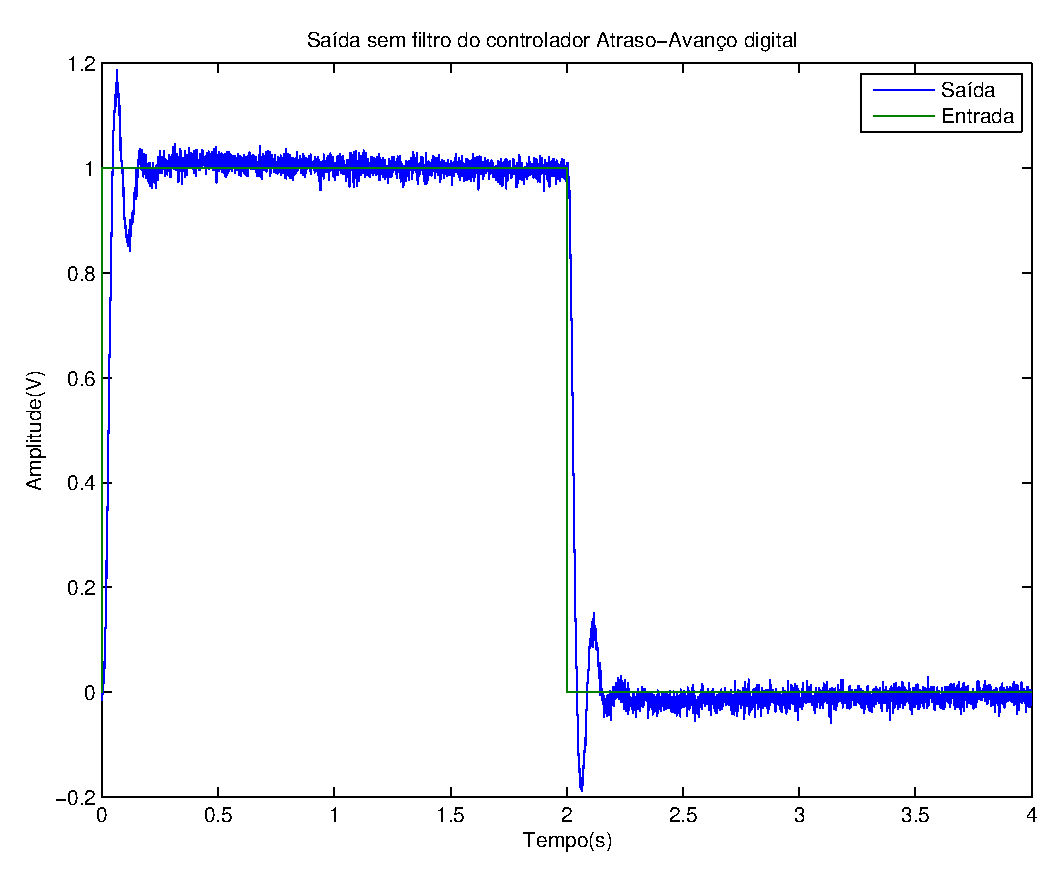
\includegraphics[width=0.8\linewidth]{ysemfiltro45}
	\caption{Resposta do controlador Avanço-Atraso 1 para onda quadrada}
	\label{fig:ysemfiltro45}
\end{figure}
\begin{figure}[H]
	\centering
	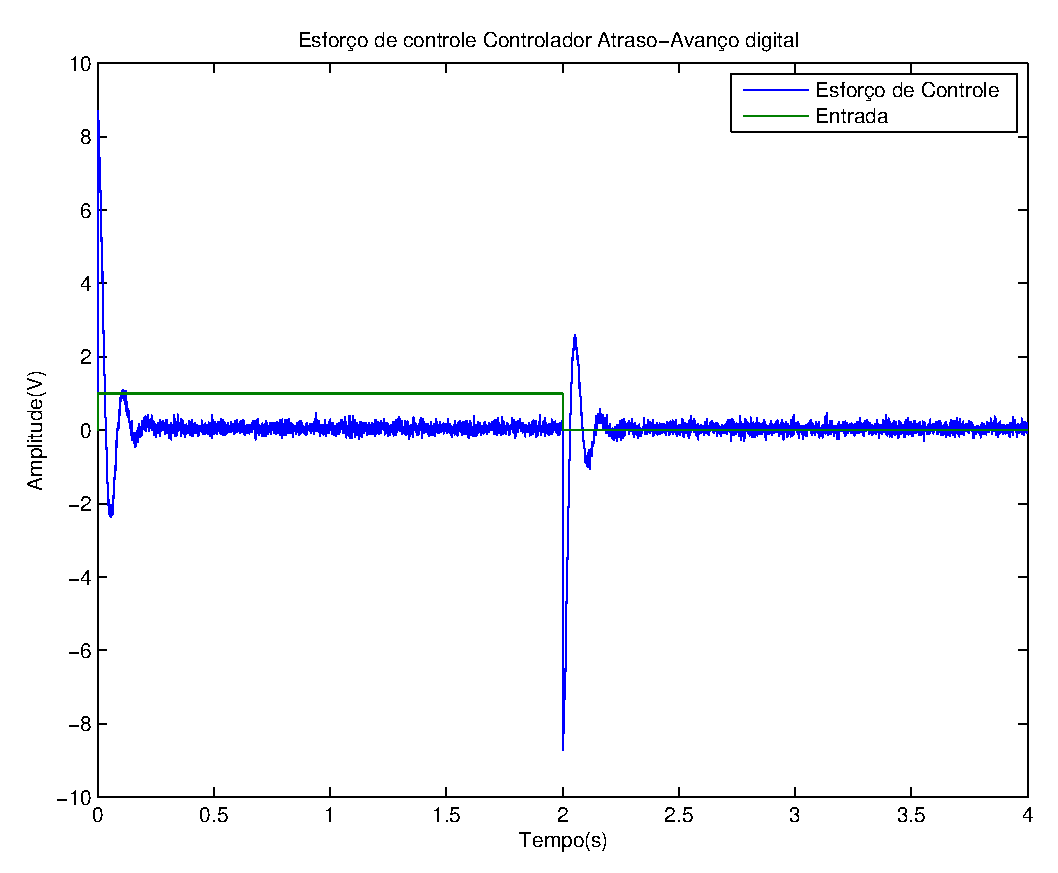
\includegraphics[width=0.8\linewidth]{upid45}
	\caption{Esforço de controle do controlador Avanço-Atraso 1 para onda quadrada}
	\label{fig:upid45}
\end{figure}
\begin{figure}[H]
	\centering
	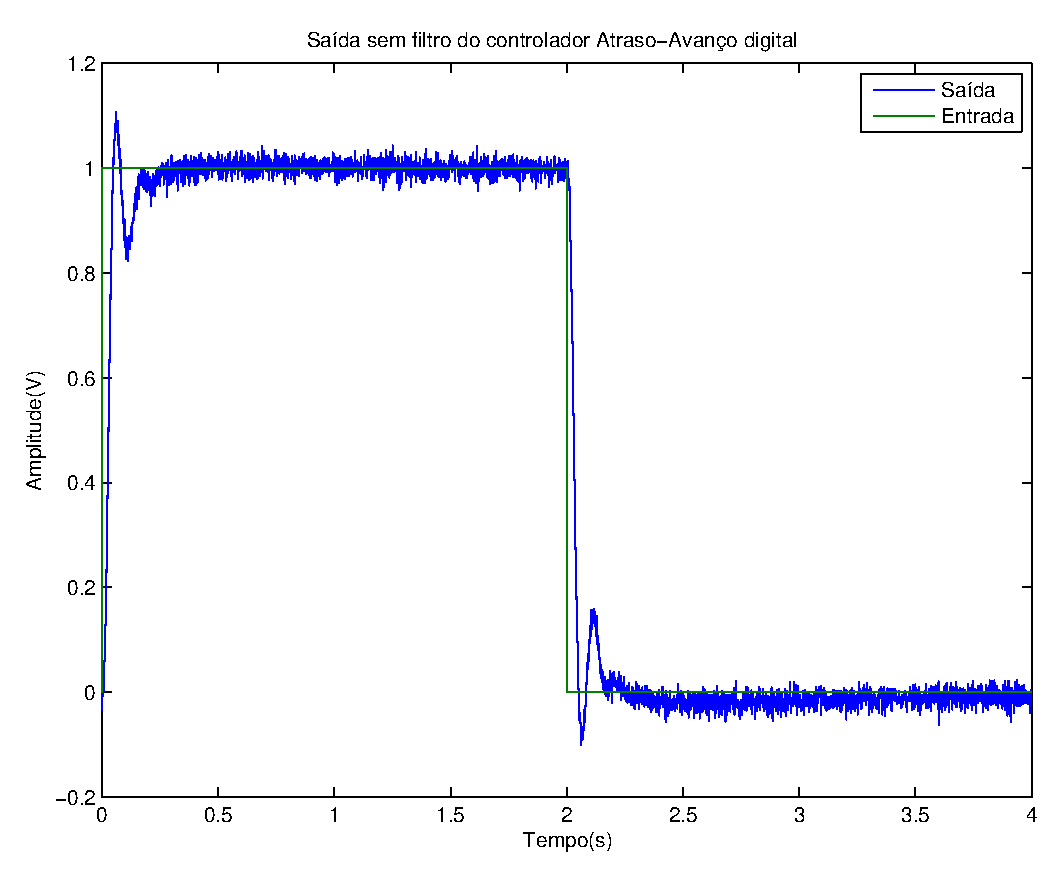
\includegraphics[width=0.8\linewidth]{ysemfiltro50}
	\caption{Resposta do controlador Avanço-Atraso 2 para onda quadrada}
	\label{fig:ysemfiltro50}
\end{figure}
\begin{figure}[H]
	\centering
	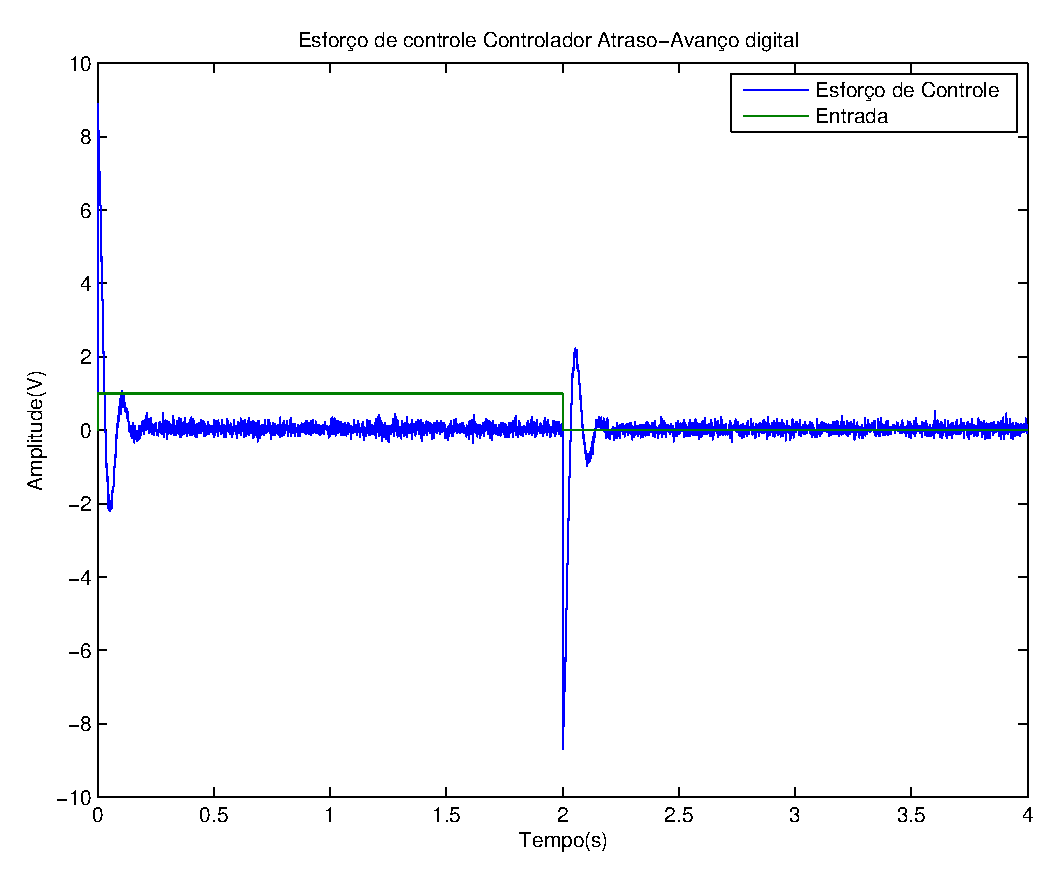
\includegraphics[width=0.8\linewidth]{upid50}
	\caption{Esforço de controle do controlador Avanço-Atraso 2 para onda quadrada}
	\label{fig:upid50}
\end{figure}
\begin{figure}[H]
	\centering
	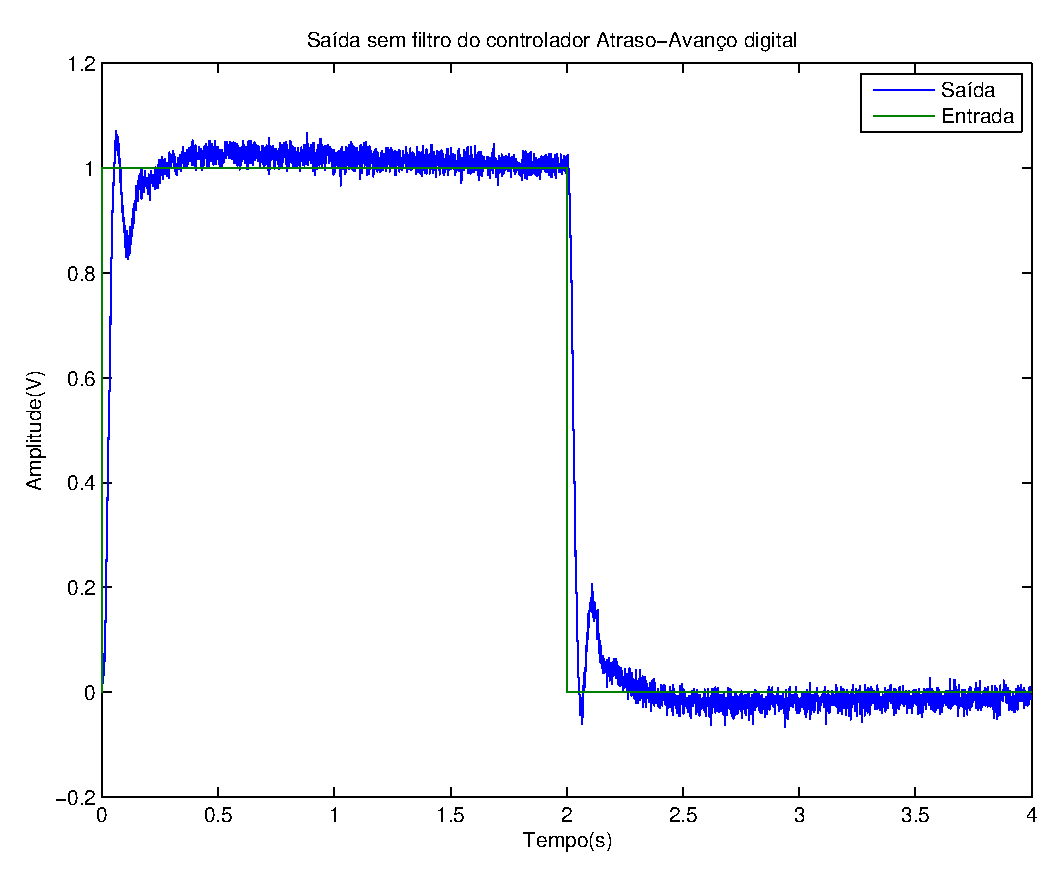
\includegraphics[width=0.8\linewidth]{ysemfiltro55}
	\caption{Resposta do controlador Avanço-Atraso 3 para onda quadrada}
	\label{fig:ysemfiltro55}
\end{figure}
\begin{figure}[H]
	\centering
	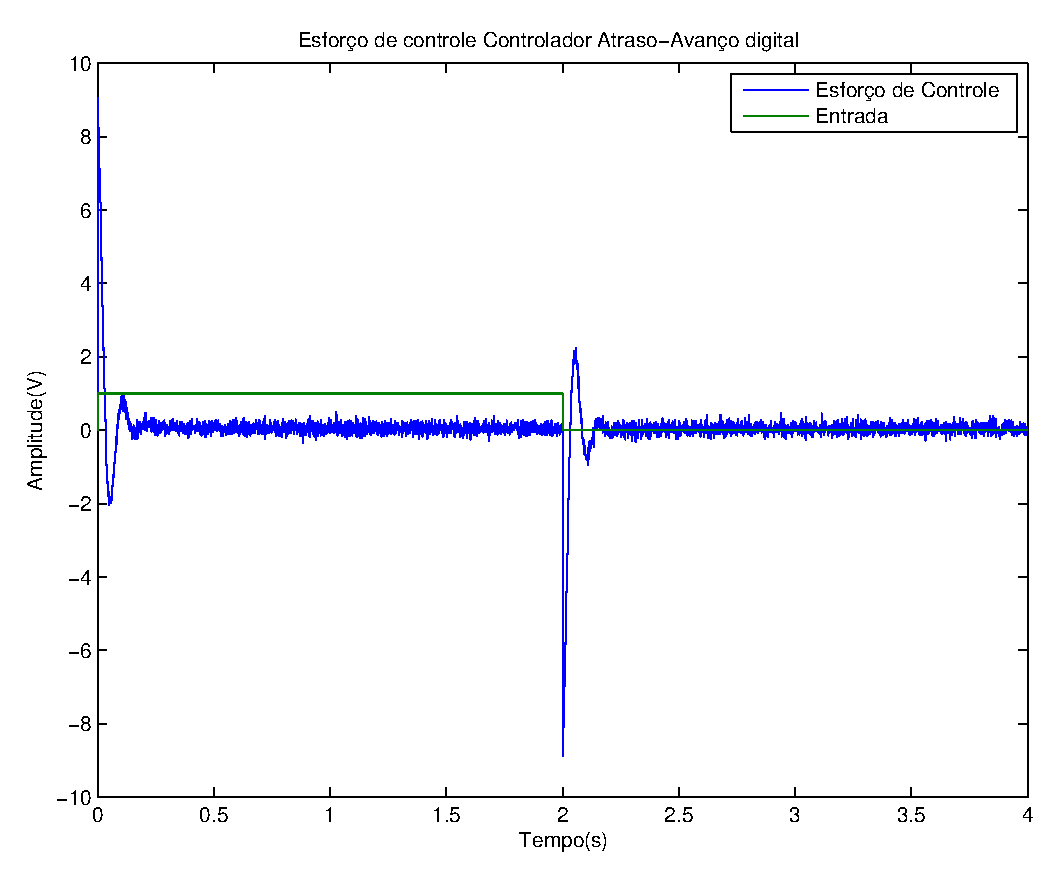
\includegraphics[width=0.8\linewidth]{upid55}
	\caption{Esforço de controle do controlador Avanço-Atraso 3 para onda quadrada}
	\label{fig:upid55}
\end{figure}

É notável que o esforço de controle apresenta um pico no momento das transições, porém o mesmo se mantém dentro dos $10V$ aceitáveis.
Com o auxílio da função \textit{stepinfo} do Matlab obtivemos alguns indicadores de desempenho para esses controladores, após filtrar a saída para eliminar os ruídos, que estão apresentados na tabela \ref{tab:avatc}
\begin{table}[H]
	\centering
	\caption{Características da resposta dos controladores Avanço-Atraso Digitais}
	\label{tab:avatc}
	\begin{tabular}{|c|c|c|c|}
		\hline Características & Controlador 1& Controlador 2& Controlador 3 \\ 
		&$M_d = 45^o$&$M_d = 50^o$&$M_d = 55^o$\\
		\hline Sobrelevação & $15.2890\%$ & $7.9620\%$ & $4.8429\%$\\
		\hline Tempo de estabilização & $0.1569s$ & $0.2576s$ & $1.2578s$\\  
		\hline Tempo de subida & $0.0294s$ & $0.0309s$ & $0.0328s$\\ 
		\hline Erro estacionário (degrau)& $0V$ & $0V$& $0.004V$\\ 
		\hline 
	\end{tabular} 
\end{table}

Como podemos ver, ao aumentar a margem de fase desejada, nós diminuímos a sobrelevação (que sempre está abaixo dos $20\%$ desejados), porém também diminuímos a velocidade de resposta do sistema.
\section{Comparação com a Resposta Simulada}
Durante as simulações realizadas para o pré roteiro \cite{bb:prelab5} nós encontramos os valores apresentados na tabela \ref{tab:avatsim}.\\
\begin{table}[H]
	\centering
	\caption{Características da resposta dos controladores Avanço-Atraso Simulados}
	\label{tab:avatsim}
	\begin{tabular}{|c|c|c|c|}
		\hline Características & Controlador 1& Controlador 2& Controlador 3 \\ 
		&$M_d = 45^o$&$M_d = 50^o$&$M_d = 55^o$\\
		\hline Sobrelevação & $12.3698\%$ & $4.0867\%$ & $3.4618\%$\\ 
		\hline Tempo de estabilização & $0.7454s$ & $1.0142s$ & $1.3472s$\\ 
		\hline Tempo de subida & $0.0503s$ & $0.0553s$ & $0.0628s$\\ 
		\hline Erro estacionário (degrau) & $0.3\%$ & $0.6\%$ & $1\%$\\ 
		\hline Erro estacionário (rampa) & $2\%$ & $2.5\%$ & $3\%$\\ 
		\hline 
	\end{tabular} 
\end{table}
Os controladores simulados apresentam um desempenho relativamente pior do que o implementado, seu tempo de estabilização é bem maior, e a diferença entre as sobrelevações não é tão grande. Essas diferenças são mais notáveis ao comparar as duas respostas (após filtrar a saída do sistema físico) como mostrado nas figuras \ref{fig:yrsim45}, \ref{fig:yrsim50} e \ref{fig:yrsim55}.
\begin{figure}[H]
	\centering
	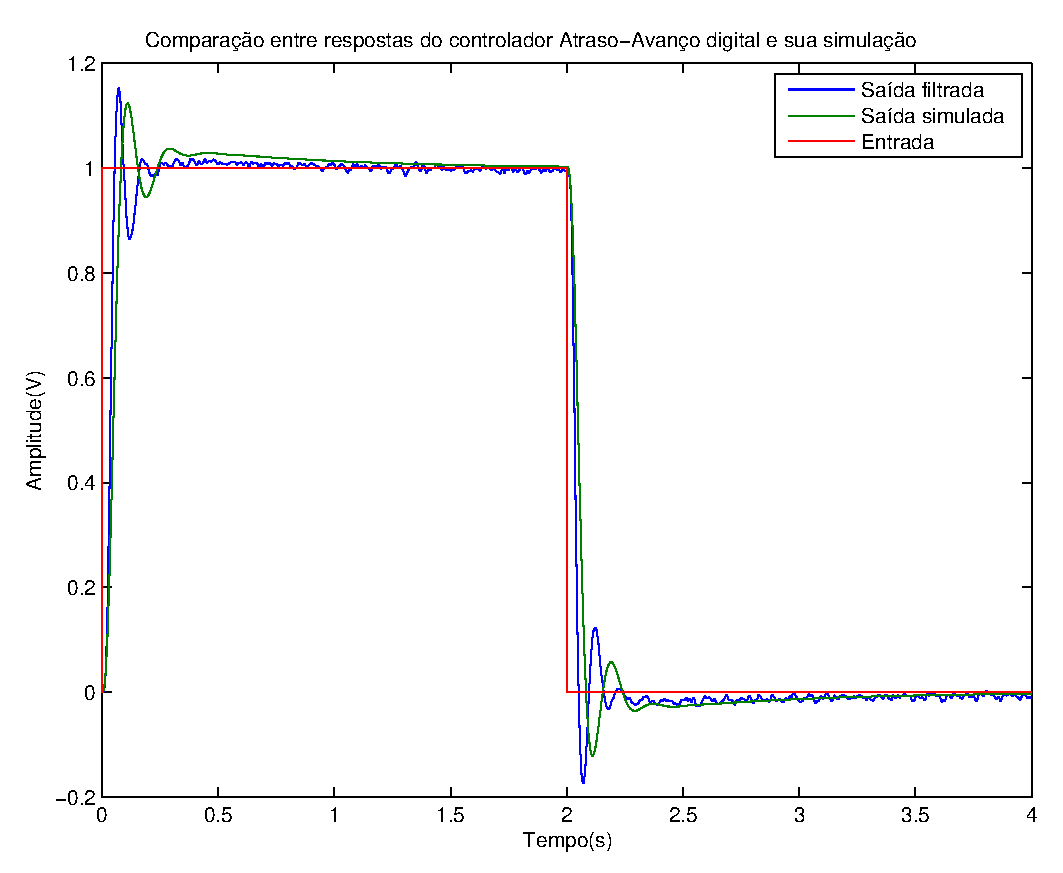
\includegraphics[width=0.8\linewidth]{yrsim45}
	\caption{Respostas dos controladores Avanço-Atraso 1 físico e simulado para onda quadrada}
	\label{fig:yrsim45}
\end{figure}
\begin{figure}[H]
	\centering
	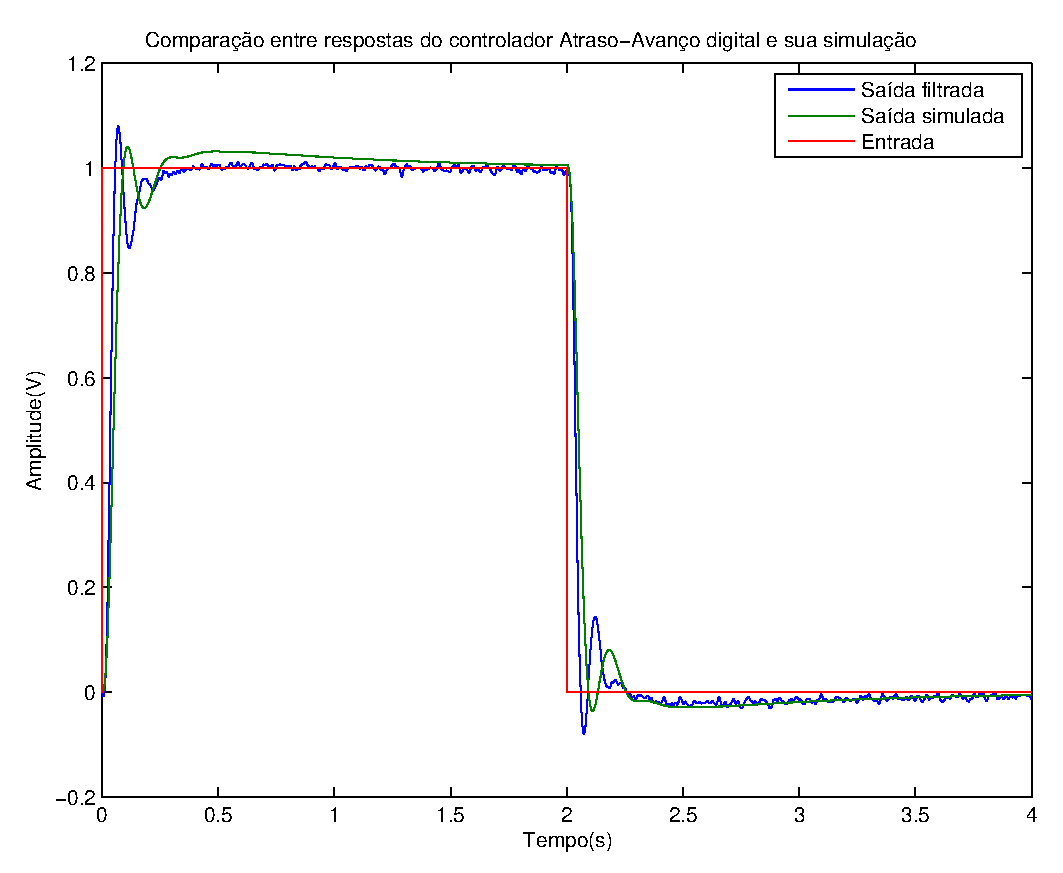
\includegraphics[width=0.8\linewidth]{yrsim50}
	\caption{Respostas dos controladores Avanço-Atraso 2 físico e simulado para onda quadrada}
	\label{fig:yrsim50}
\end{figure}
\begin{figure}[H]
	\centering
	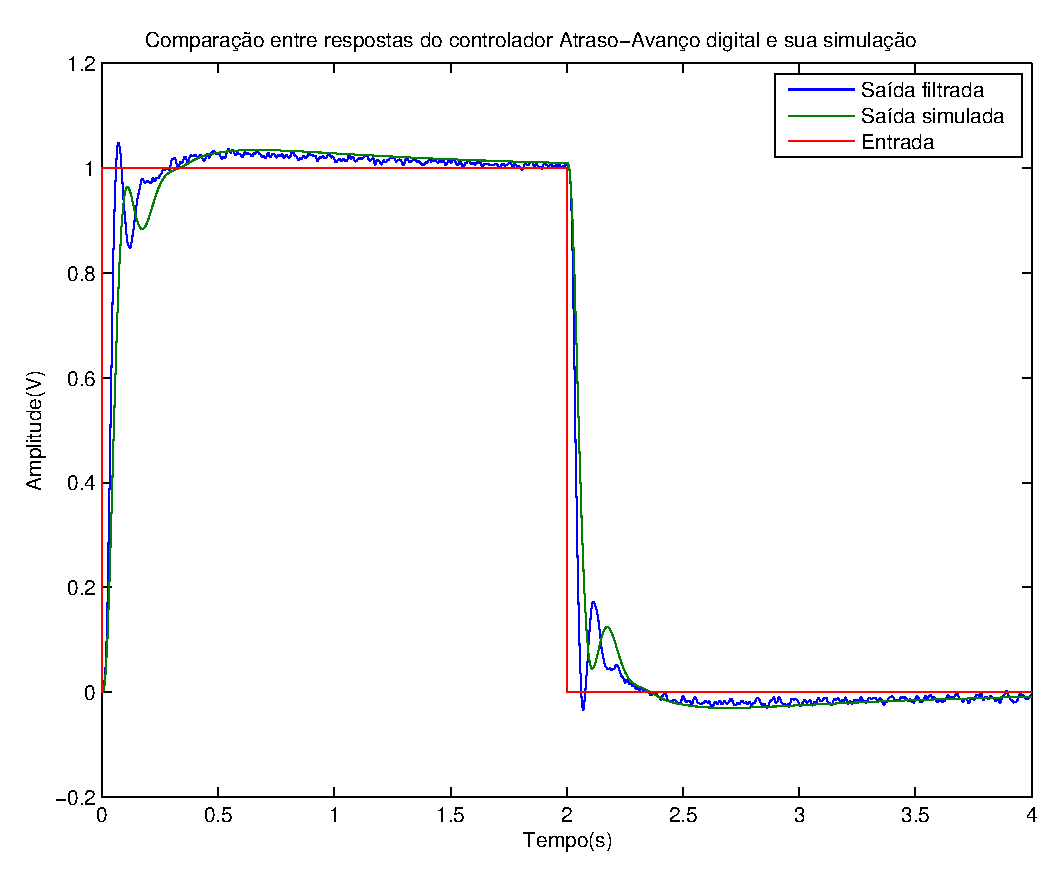
\includegraphics[width=0.8\linewidth]{yrsim55}
	\caption{Respostas dos controladores Avanço-Atraso 3 físico e simulado para onda quadrada}
	\label{fig:yrsim55}
\end{figure}
Acreditamos que essas diferenças se dão, em grande parte, do fato da planta calculada diferir da planta física.

Podemos ver também que os esforços de controle dos dois controladores são bastante semelhantes, como pode ser visto nas figuras \ref{fig:ursim45}, \ref{fig:ursim50} e \ref{fig:ursim55}.
\begin{figure}[H]
	\centering
	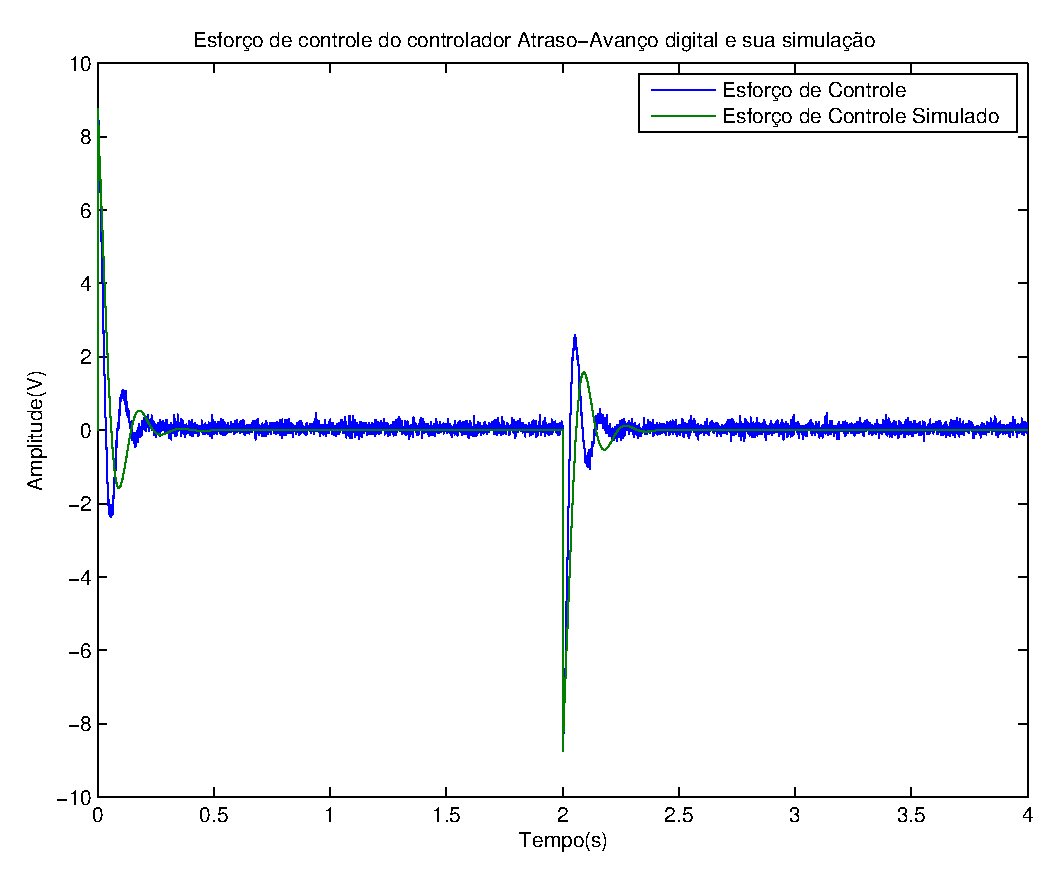
\includegraphics[width=0.8\linewidth]{ursim45}
	\caption{Esforços de controle dos controladores Avanço-Atraso 1 físico e simulado para onda quadrada}
	\label{fig:ursim45}
\end{figure}
\begin{figure}[H]
	\centering
	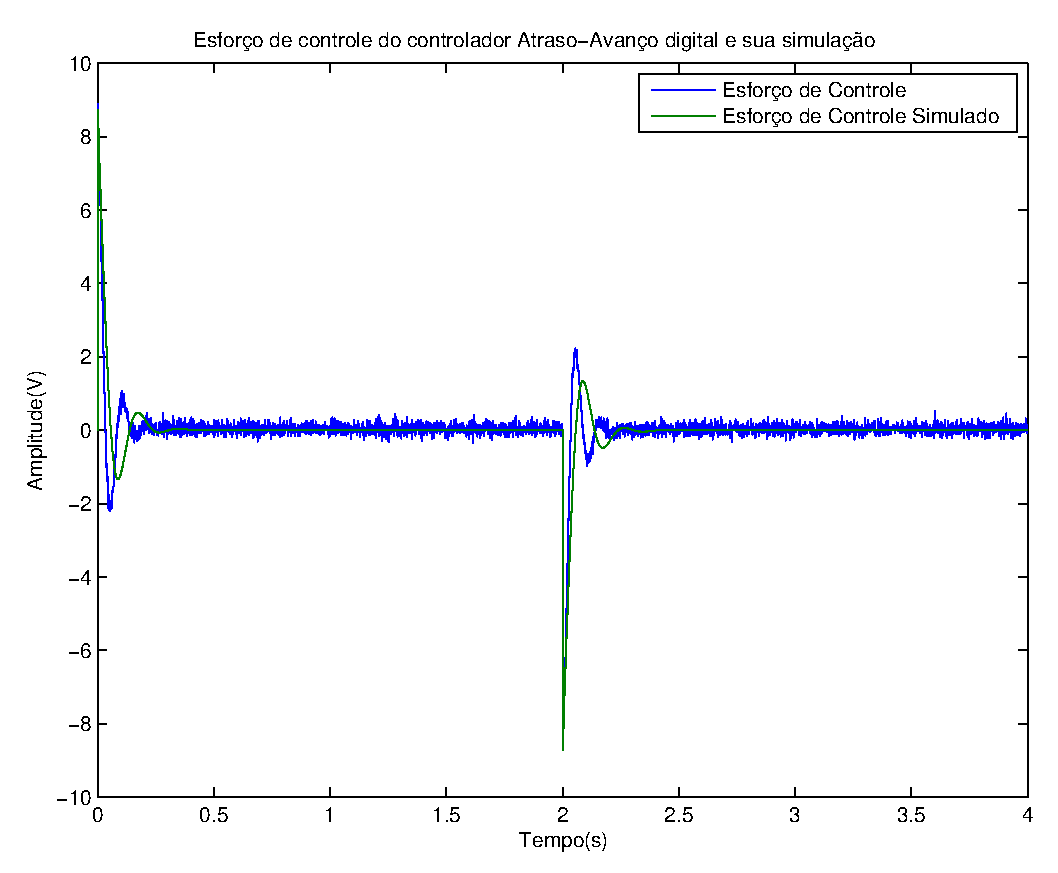
\includegraphics[width=0.8\linewidth]{ursim50}
	\caption{Esforços de controle dos controladores Avanço-Atraso 2 físico e simulado para onda quadrada}
	\label{fig:ursim50}
\end{figure}
\begin{figure}[H]
	\centering
	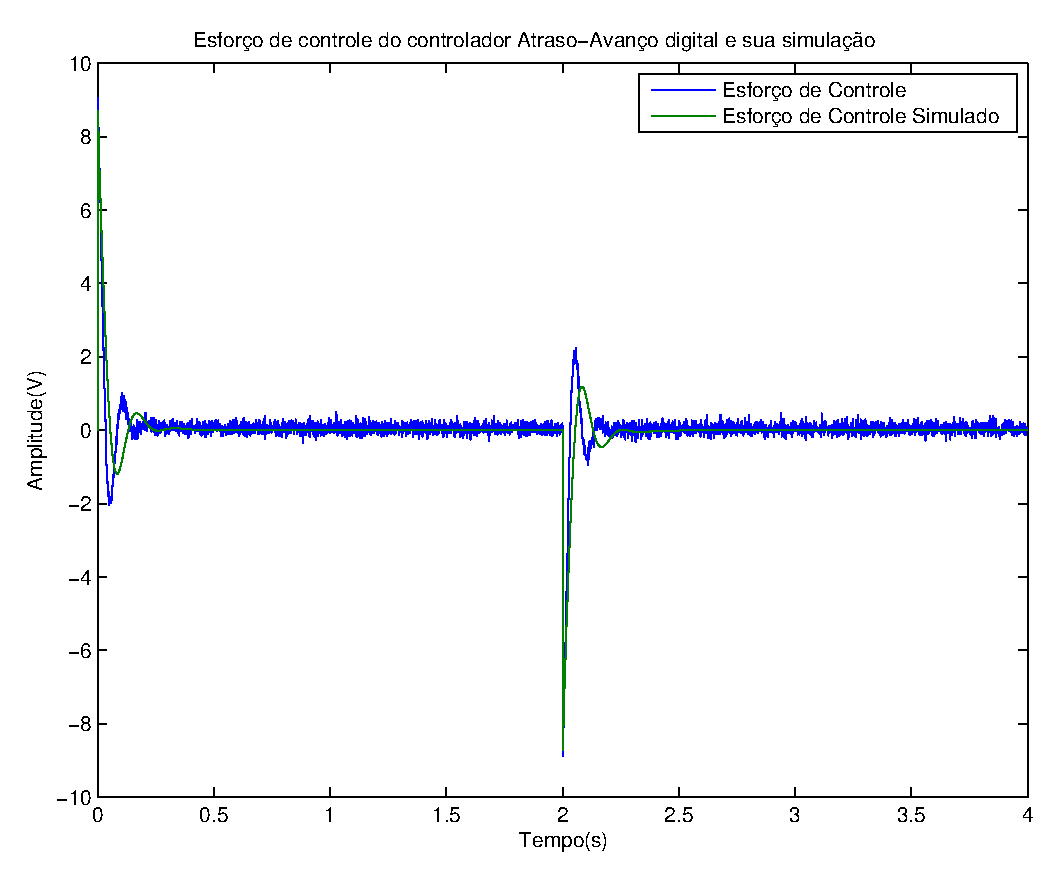
\includegraphics[width=0.8\linewidth]{ursim55}
	\caption{Esforços de controle dos controladores Avanço-Atraso 3 físico e simulado para onda quadrada}
	\label{fig:ursim55}
\end{figure}

\section{Comparação com outros Controladores}
Por fim, mostramos na figura \ref{fig:yrcomp} uma comparação entre os resultados deste controlador analógico e os dos melhores controladores implementados nos relatórios anteriores: os controladores digitais proporcional com sobrelevação de 2\% e PID projetado pelo método Ziegler-Nichols do experimento 3 \cite{bb:lab3} e o controlador PID analógico do experimento 4 \cite{bb:lab4}.
\begin{figure}[H]
	\centering
	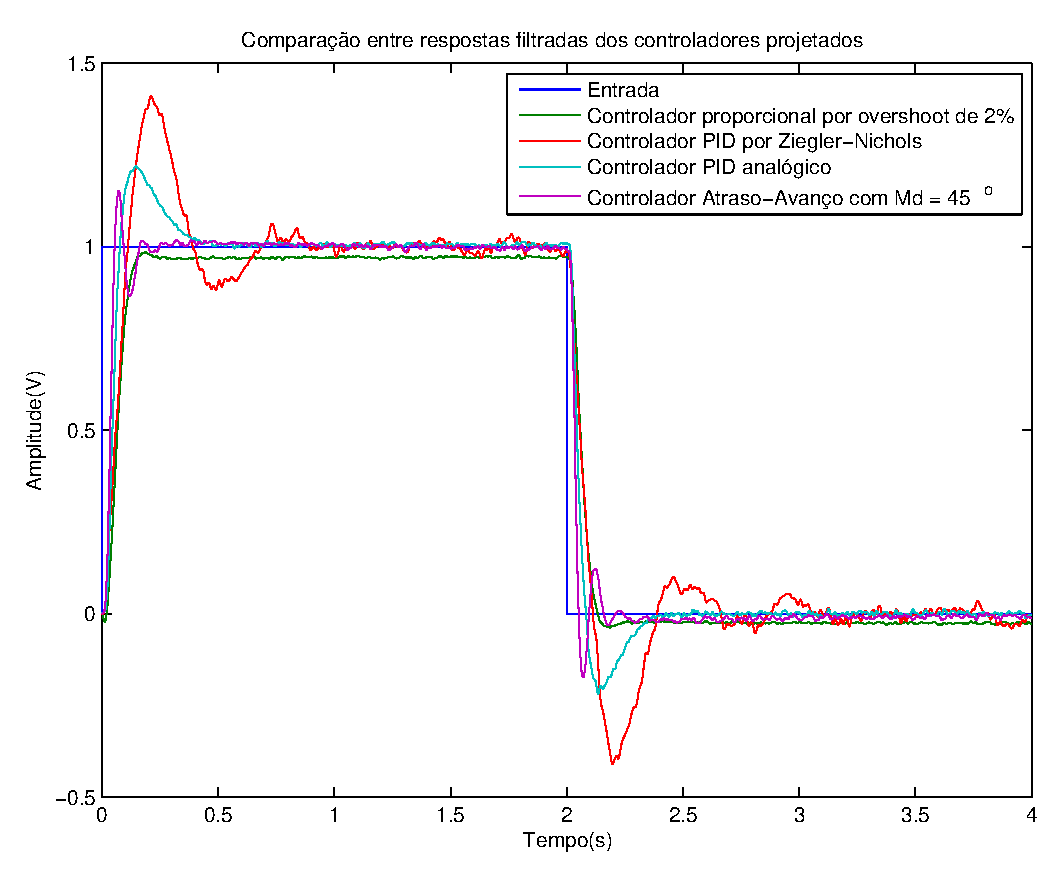
\includegraphics[width=0.8\linewidth]{yfrcomp}
	\caption{Comparação entre as respostas filtradas dos controladores para onda quadrada}
	\label{fig:yrcomp}
\end{figure}
A diferença em tempo de estabilização do controlador Avanço-Atraso é notável, apresentado a melhor resposta até agora. O único outro controlador que se aproxima do mesmo é o controlador proporcional projetado durante o experimento 3 \cite{bb:lab3}, porém este apresenta um erro estacionário maior, especialmente quando a entrada é uma rampa.

\begin{thebibliography}{widestlabel}
	\bibitem{bb:roteiro}{Roteiro do experimento disponibilizado para os alunos}
	\bibitem{bb:lab2}{KIAN, Marcelli; OLIVEIRA, Daniel. \textit{Relatório - Experimento 2:} Identificação de plantas eletrônicas.}
	\bibitem{bb:lab3}{KIAN, Marcelli; OLIVEIRA, Daniel. \textit{Relatório - Experimento 3:} Controle de plantas eletrônicas utilizando um controlador PID digital.}
	\bibitem{bb:lab4}{KIAN, Marcelli; OLIVEIRA, Daniel. \textit{Relatório - Experimento 4:}  Controle de plantas eletrônicas utilizando um controlador PID analógico.}
	\bibitem{bb:prelab5}{KIAN, Marcelli; OLIVEIRA, Daniel. \textit{Pré Relatório - Experimento 5:}  Controle de plantas eletrônicas utilizando um controlador atraso-avanço digital.}
\end{thebibliography}
\end{document}

